\begin{figure}[!htbp]
  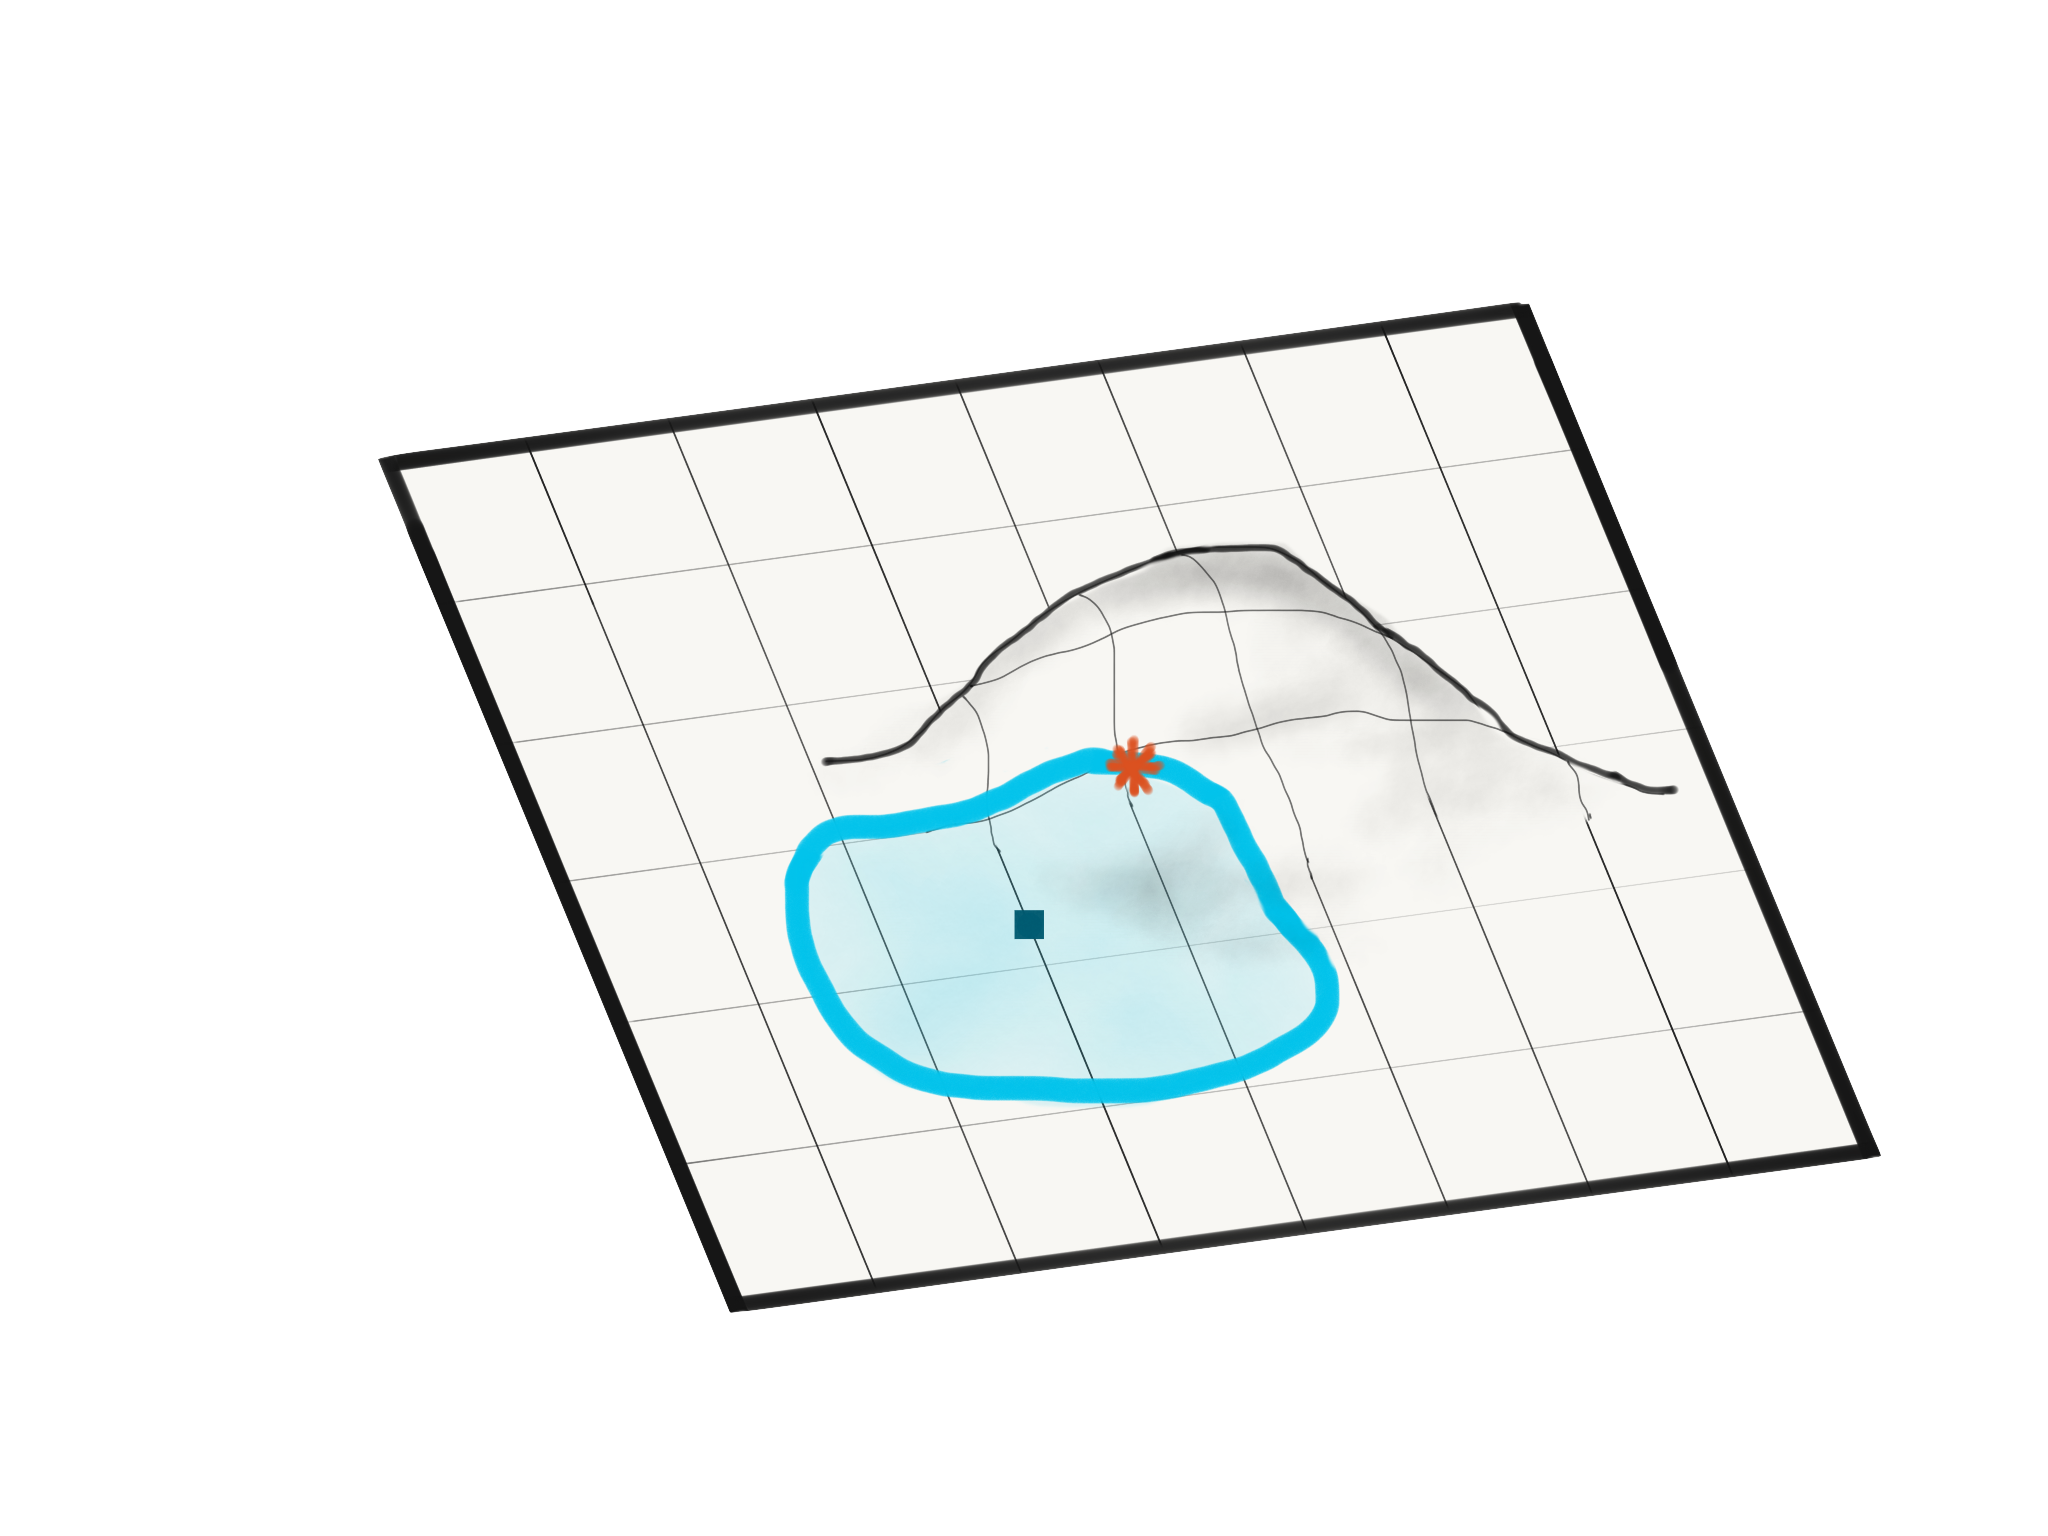
\includegraphics[width=0.8\textwidth]{img/baldwin_effect.png}
  \captionsetup{singlelinecheck=off,justification=raggedright}
  \caption{The Baldwin effect postulates that learning --- in evolutionary terms phenotypic plasticity or, equivalently and more explicitly, local search in the phenotype space --- biases evolutionary search to allow advantageous phenotypic features originally acquired via phenotypic plasticity to encoded into the genetic representation \cite{Downing2010TheNetworks}. In the first phase of the Baldwin effect, advantageous phenotypic features discovered by local search in the phenotype space increase the fitness of individuals proximal to that phenotype. Phenotypic plasticity is illustrated in the above cartoon, where the phenotype space is depicted as a three dimensional surface with points on the surface representing different phenotypes and the height of the surface denoting the fitness of the phenotypes at those points. In the illustration, the dark blue square represents the phenotype originally mapped to by the genetic representation of an individual, the blue shaded region represents the region of the phenotype space searched via phenotypic plasticity, and the red star represents a high fitness phenotypic variant reached via phenotypic plasticity. The fitness boost gained from phenotypic proximity to a high fitness solution biases evolutionary search to continue exploring that region of the instead of proceeding in other directions. In the second phase of the Baldwin effect, that continued evolutionary search promotes phenotypic features discovered by phenotypic plasticity are encoded into the genetic representation. Cost or unreliability of generating the advantageous phenotypic feature via phenotypic plasticity provides evolutionary pressure that favors genetic encoding of that phenotypic feature. In the case of indirect genotype to phenotype mappings, a direct genetic encoding of the feature discovered via phenotypic plasticity might not exist; however, genomes that map to phenotypes closer to the phenotypic feature discovered by plasticity --- which support attainment of the phenotypic feature by reducing the cost or increasing the reliability of acquiring that feature via plasticity, providing ``scaffolding'' for the local phenotypic search --- may still arise and will be selected for \cite{DowningHeterochronousBaldwinism}.}
     \label{fig:baldwin_effect}
\end{figure}